\documentclass[crop,tikz]{standalone}
\usetikzlibrary{backgrounds}
\colorlet{blue}{cyan}
\tikzset{
  inverted/.style = {
    every path/.style = {draw=white,text=white},
    background rectangle/.style={fill},
    show background rectangle
  }
}

\tikzset{>=latex}

\begin{document}
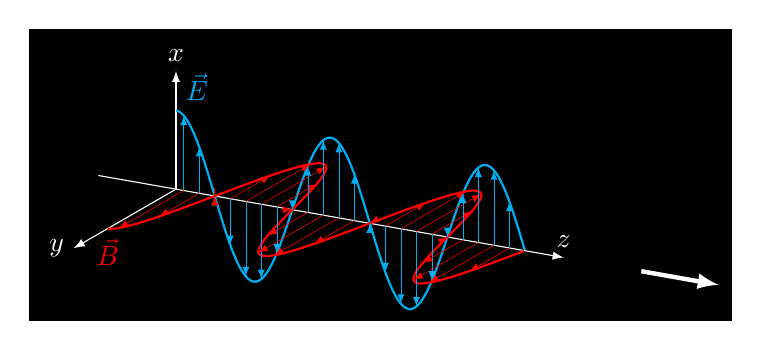
\begin{tikzpicture}[inverted,x={(-10:1cm)},y={(90:1cm)},z={(210:1cm)}]
  % axis
  \draw[->] (-1,0,0) -- (5,  0,0) node[above] {$z$};
  \draw[->] ( 0,0,0) -- (0,1.5,0) node[above] {$x$};
  \draw[->] ( 0,0,0) -- (0,0,1.5) node[left ] {$y$};
  % propagation
  \draw[->,ultra thick] (6,0,0) -- (7,0,0);
  % waves
  \draw[blue,thick] plot[domain=0:4.5,samples=200] (\x,{cos(deg(pi*\x))},0);
  \draw[red ,thick] plot[domain=0:4.5,samples=200] (\x,0,{cos(deg(pi*\x))});
  % arrows
  \foreach \x in {0.1,0.3,...,4.4} {
    \draw[->,help lines,blue] (\x,0,0) -- (\x,{cos(deg(pi*\x))},0);
    \draw[->,help lines,red ] (\x,0,0) -- (\x,0,{cos(deg(pi*\x))});
  }
  % labels
  \node[blue,above right] at (0,1,0) {$\vec{E}$};
  \node[red,below] at (0,0,1) {$\vec{B}$};
\end{tikzpicture}
\end{document}
